\chapter{Implementación\label{cap:implementacion}}

En este capítulo se explica cómo se han implementado los dos componentes principales de la aplicación, tal y como se diseñaron y estructuraron en el capítulo \ref{cap:disenho}: un servicio web (el \gls{back-end}) y una interfaz web (el \gls{front-end}).
Se detalla además qué documentación se ha generado en esta fase, tanto interna del proyecto como para el usuario final de la aplicación.

\section{Back-End\label{sec:imp:back_end}}

Para la implementación del \gls{back-end} se han utilizado las librerías en \textit{JavaScript} mencionadas en la sección~\ref{ssec:dp:back-end}.
Así, se ha creado una \gls{API} \gls{REST} con la ayuda de la librería \textit{Express}, sobre el \gls{framework} \textit{node.js}.
Adicionalmente, se hace uso de la librería \textit{Async} para facilitar el manejo de funciones asíncronas, y de \textit{nodemon} para cubrir la función de supervisor descrita en el diseño.
Finalmente, se ha encapsulado el componente dentro de un servicio que se inicia automáticamente al arrancar el ordenador, haciendo que el \gls{back-end} esté activo siempre que el servidor de la sonda de red se encuentre operativo.

\begin{figure}[!htp]
  \centering
  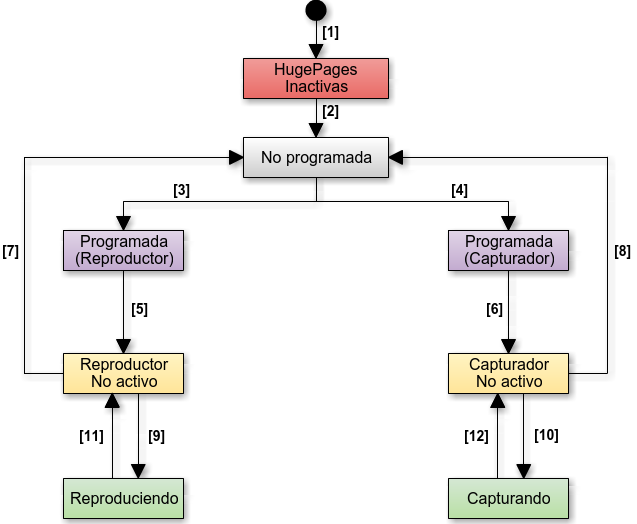
\includegraphics[width=\textwidth,clip=true]{fpga_estado}
  \caption{Máquina de Estados Finitos del \gls{back-end}.}
  \label{fig:fpga_estado}
\end{figure}

El objetivo principal del \gls{back-end} es formalizar el estado de la \gls{FPGA}, permitiendo así su consulta y modificación.
Para programar este aspecto, se han modelado los posibles estados internos del sistema en una Máquina de Estados Finitos (ver Figura~\ref{fig:fpga_estado}).
Las transiciones existentes entre los estados son:
\begin{enumerate}[label={\bfseries [\arabic*]}]
  \item Iniciar el servidor sin seleccionar la opción de arrancar con \textit{HugePages} habilitadas.
  \item Reiniciar el servidor, seleccionando la opción de arrancar con \textit{HugePages} habilitadas.
  \item Programar la \gls{FPGA} en modo reproductor con el \gls{bitstream} correspondiente y reiniciar el servidor.
  \item Programar la \gls{FPGA} en modo capturador con el \gls{bitstream} correspondiente y reiniciar el servidor.
  \item Montar la \gls{FPGA} sobre el servidor.
  \item Montar la \gls{FPGA} sobre el servidor.
  \item Reiniciar el servidor.
  \item Reiniciar el servidor.
  \item Ordenar a la sonda reproducir una \gls{traza}.
  \item Ordenar a la sonda capturar una \gls{traza}.
  \item Reproducción finalizada, o porque se ha acabado el contenido de la \gls{traza} o porque ha sido detenida el usuario.
  \item Captura finalizada, o porque se ha capturado todo lo que se quería o porque es detenida por el usuario.
\end{enumerate}

\begin{figure}[!htp]
  \centering
  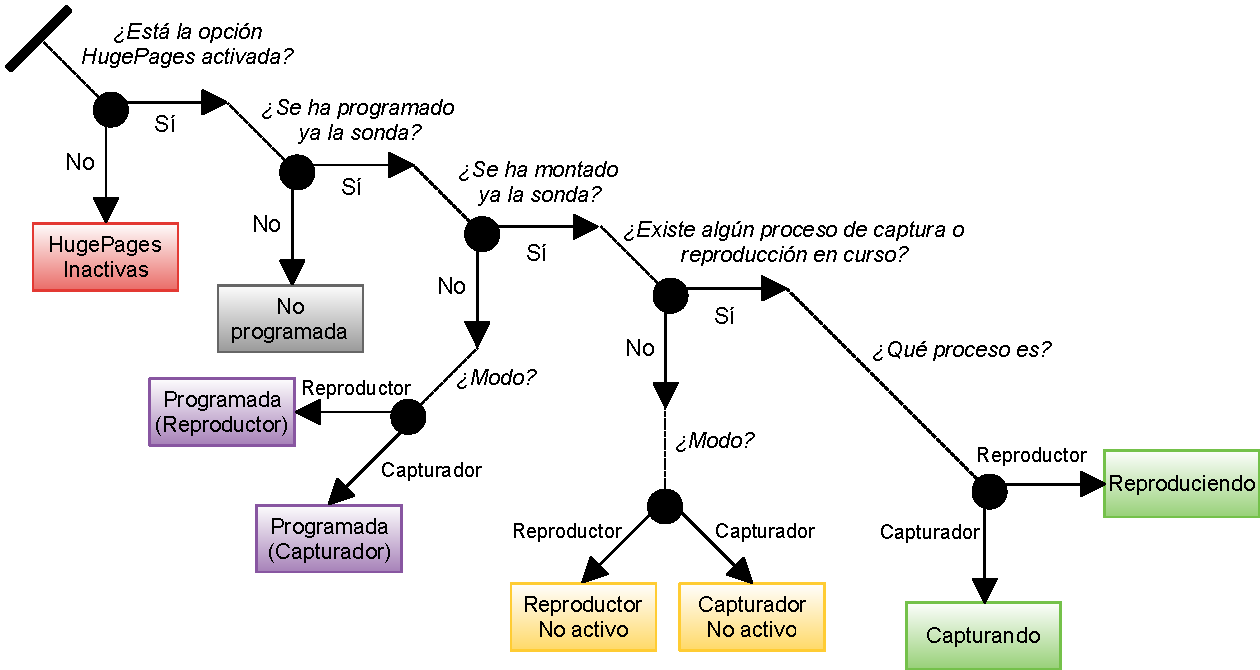
\includegraphics[width=0.75\textwidth,clip=true]{arbol_decision}
  \caption{Árbol de decisión para determinar el estado de la \gls{FPGA}.}
  \label{fig:arbol_decision}
\end{figure}

Para conocer el estado actual de esta máquina de estados y verificar qué operaciones puede realizar la \gls{FPGA}, se plantearon dos alternativas: mantener sincronizadas la sonda de red y el servicio web, de forma que el se detectase cualquier cambio en la \gls{FPGA} y el servicio web almacenase el estado de forma persistente, o que cada vez que se necesitase conocer el estado de la sonda se determinase de nuevo.
Se ha elegido la segunda opción, ya que evita que pueda haber incoherencias entre el estado real de la \gls{FPGA} y el guardado en el servicio.
Además, así el servicio web tendrá que consultar a la sonda solo en caso de que haya una petición dirigida al \gls{back-end}, no utilizando recursos monitorizando la \gls{FPGA} si no ha sido invocado.
Se ha implementado, siguiendo esta segunda opción, un árbol de decisión binario que determina el estado actual de la \gls{FPGA} mediante consultas a la propia sonda y al sistema (ver Figura~\ref{fig:arbol_decision}).

Los archivos de código más relevantes de la implementación del \gls{back-end} se muestran en la Figura~\ref{fig:arbol_codigo}, siendo \textit{server.js} el principal. Este se encarga de lanzar el grupo de procesos que responde a las peticiones del \gls{front-end}, delegándolas según corresponda a uno de los tres módulos existentes.
Cada uno de estos módulos consta de dos archivos en \textit{JavaScript}.
El primero, con el nombre del propio módulo, contiene las funciones de la \gls{API} del \gls{back-end} (ver Figura~\ref{fig:arbol_metodos}).
El segundo fichero, con el nombre del módulo seguido de \textit{\_utils}, recoge funciones auxiliares.
Por último, las funciones comunes a todos los módulos han sido codificadas en un único archivo, \textit{\_common.js}.

\begin{figure}[!htp]
  \begin{center}
    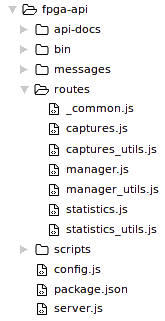
\includegraphics[width=0.3\textwidth,clip=true]{capturas/arbol_backend}
    \hspace{1cm}
    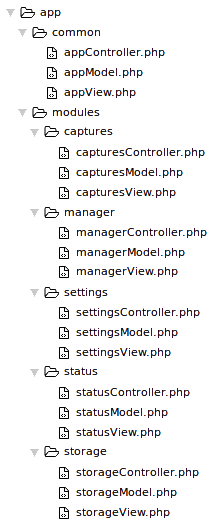
\includegraphics[width=0.3\textwidth,clip=true]{capturas/arbol_frontend}
  \caption{Árboles con los principales archivos de código del \gls{back-end} (a la izquierda) y del \gls{front-end} (a la derecha).}
  \label{fig:arbol_codigo}
  \end{center}
\end{figure}

\begin{figure}[!htp]
  \centering
  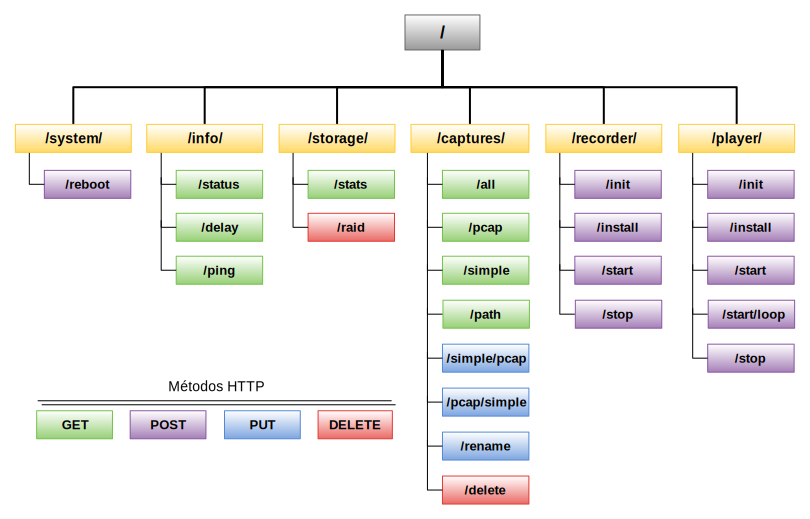
\includegraphics[width=\textwidth,clip=true]{arbol_metodos}
  \caption{Métodos públicos del \gls{servicioweb} \gls{FPGA}.}
  \label{fig:arbol_metodos}
\end{figure}

\section{Front-End\label{sec:imp:front_end}}

Para la implementación del \gls{front-end} se ha partido del \gls{framework} propio desarrollado, utilizándose las herramientas en \textit{JavaScript}, \textit{CSS} y \textit{HTML5} descritas en la sección~\ref{ssec:dp:back-end}.
Así, se ha hecho uso de la librería \textit{jQuery} para la gestión de los elementos dinámicos de la interfaz web y de \textit{Chart.js} para la realización de gráficas sobre el rendimiento y el almacenamiento disponible.

Un aspecto que se ha considerado importante, en términos de usabilidad, es que el usuario pueda conocer en todo momento el estado del sistema.
Con este objetivo en mente, toda acción del usuario tiene como respuesta una confirmación visual del resultado de la misma.
Las operaciones mayores implican una actualización o cambio de la página actual, mientras que para las acciones menores se han utilizado notificaciones emergentes, para las cuales se han utilizado las librerías \textit{Bootstrap Notify} y \textit{Animate.css}.


Internacionalización, inglés y español
\textit{gettext}

diseño \textit{responsive}, comentado en la sección~\label{sec:dis:interfaz_web},
Resultado Capturas diseño responsive, (misma página desde dos sitios)~\ref{fig:captura:movil}
\textit{Bootstrap},
\textit{Bootstrap table}

\begin{figure}[!htp]
  \centering
  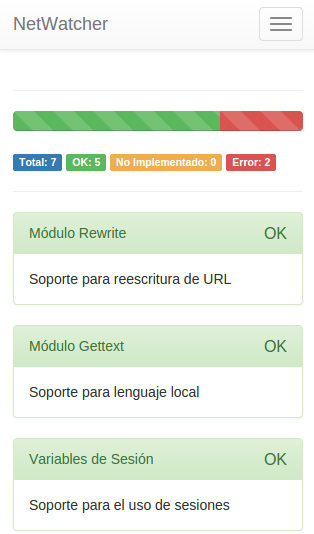
\includegraphics[width=0.4\textwidth,clip=true]{capturas/estado_movil}
  \caption{Página de la aplicación visualizada desde un dispositivo móvil.}
  \label{fig:captura:movil}
\end{figure}

Temas (captura algún temas)~\ref{fig:captura:oscuro}
colección de temas \textit{Bootswatch}

\begin{figure}[!htp]
  \centering
  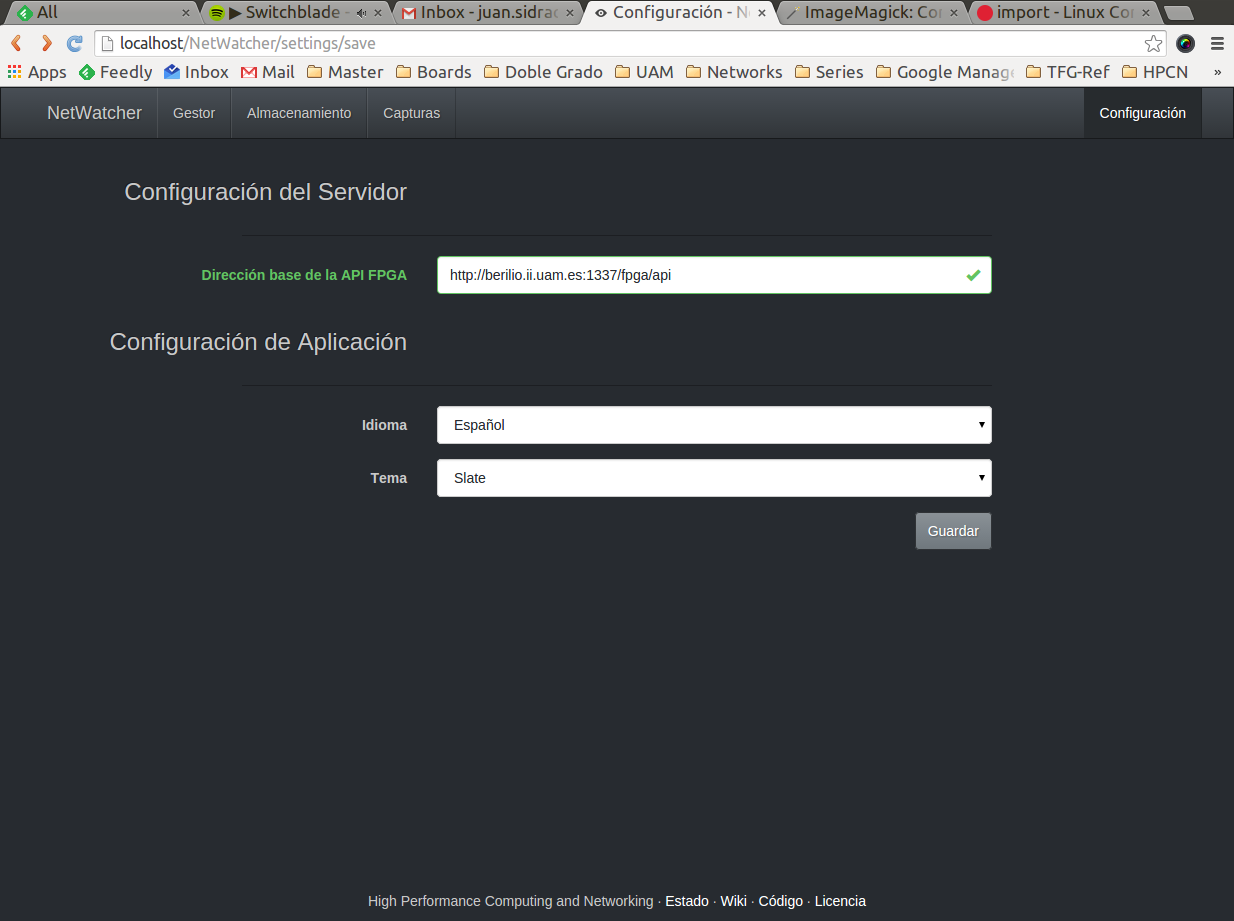
\includegraphics[width=0.95\textwidth,clip=true]{capturas/configuracion_tema_oscuro}
  \caption{Página de la aplicación con un tema oscuro seleccionado.}
  \label{fig:captura:oscuro}
\end{figure}

Los submódulos (páginas) de la interfaz web se estructuran internamente siguiendo el modelo de arquitectura modelo-vista-controlador, implementado de forma abstracta en el módulo \textit{common}.
Los archivos de código más relevantes de esta implementación del \gls{front-end} se muestran en la Figura~\ref{fig:arbol_codigo}.
Así, cada uno de los submódulos consta tres archivos de código: \textit{Model}, \textit{View} y \textit{Controller}.

\section{Documentación \label{sec:imp:docs}}

Se ha creado distinta documentación del proyecto según a quién esté dirigida.
Por un lado, se ha escrito un manual de usuario (disponible en el apéndice~\ref{extra:manual_de_usuario}), que pretende ser una guía completa y suficiente para la instalación, configuración y uso de la aplicación.
Adicionalmente, se han publicado en el repositorio de \textit{GitHub} del proyecto (\url{github.com/JSidrach/NetWatcher}) una serie de páginas en formato \textit{wiki} (ver Figura~\ref{fig:captura:wiki}). Estas páginas, en inglés, recogen los aspectos más importantes de la aplicación, tanto para el usuario final como para desarrolladores.

\begin{figure}[!htp]
  \centering
  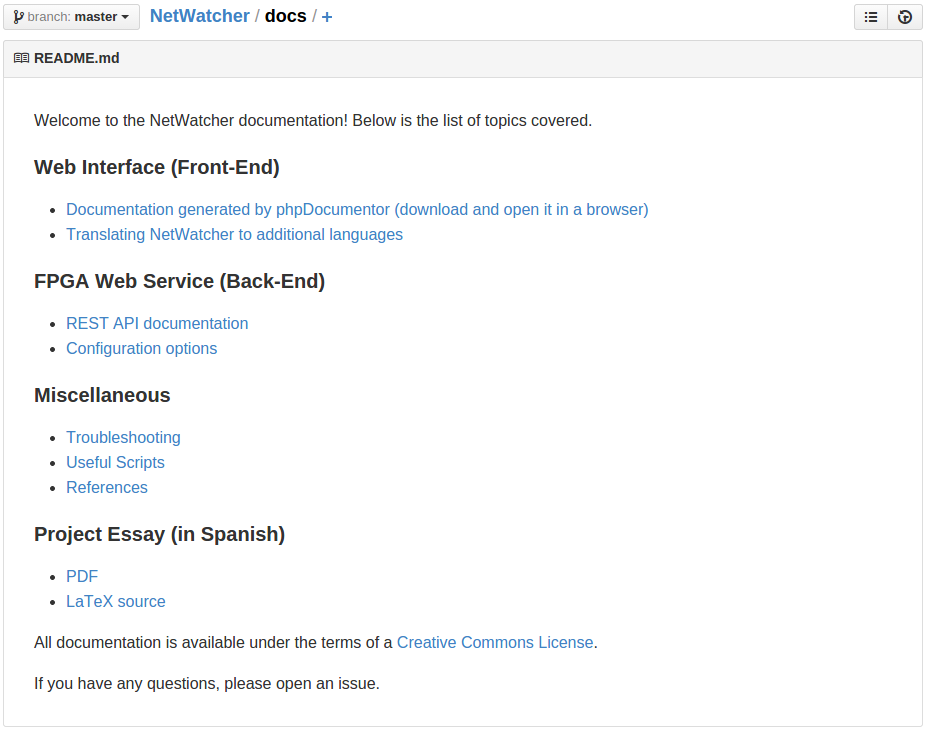
\includegraphics[width=0.95\textwidth,clip=true]{graphics/capturas/github_docs}
  \caption{Captura de una de las páginas de la wiki del proyecto.}
  \label{fig:captura:wiki}
\end{figure}

A nivel específico de desarrollador, se han utilizado dos herramientas para crear la documentación interna, accesible a través del navegador y en inglés.
La documentación del \gls{front-end} se ha generado con \textit{phpDocumentor} (ver Figura~\ref{fig:captura:docsfrontend}), y la del \gls{back-end} con \textit{apiDoc}.
Esta última se adjunta también, traducida al español, en el apéndice~\ref{extra:api_servicio_web_fpga}.
Por último, en el apéndice~\ref{extra:frameworkDesarrollado} se explican la arquitectura y funcionalidad del \gls{framework} base para el \gls{front-end}.

\begin{figure}[!htp]
  \centering
  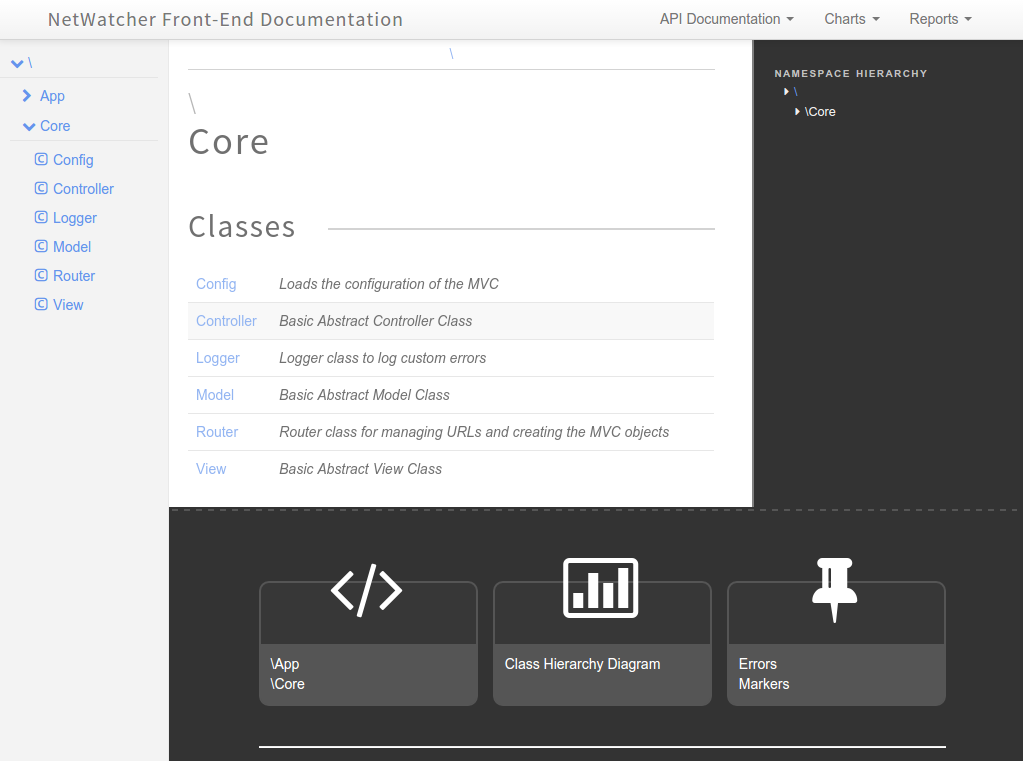
\includegraphics[width=0.95\textwidth,clip=true]{graphics/capturas/docs_frontend}
  \caption{Documentación web del \gls{front-end}.}
  \label{fig:captura:docsfrontend}
\end{figure}
